% !TEX program = pdflatex
\documentclass[aspectratio=169, 10pt]{beamer}

% ══════════════════════════════════════════════════════════════
%  COLETOR MULTIBASE DE ARTIGOS CIENTÍFICOS
%  Preâmbulo derivado de apresentacao.tex.
%  Imagens: background_first.jpeg (capa), background.jpeg (seções)
%  Figuras: pasta figuras/ (geradas por gerar_graficos.py)
% ══════════════════════════════════════════════════════════════

% ── DADOS DA APRESENTAÇÃO ────────────────────────────────────
\newcommand{\apTitulo}{Coletor Multibase de Artigos Científicos}
\newcommand{\apSubtitulo}{Aquisição em APIs acadêmicas e classificação com LLM local}
\newcommand{\apAutores}{Arthur Cadore Matuella Barcella}
\newcommand{\apInstituicao}{ITA -- TE-251 -- Projeto final}
\newcommand{\apRodape}{COLETOR DE ARTIGOS}
\newcommand{\apRodapeCentro}{Como o coletor funciona}
\newcommand{\apData}{\today}

% ── Tema base (minimal) ──────────────────────────────────────
\usetheme{default}
\setbeamertemplate{navigation symbols}{}
\setbeamertemplate{itemize item}{\scriptsize\raise1pt\hbox{\color{radarcyan}$\bullet$}}
\setbeamertemplate{itemize subitem}{\tiny\raise1pt\hbox{\color{radargreen}$\circ$}}
\setbeamertemplate{itemize subsubitem}{\tiny\raise1pt\hbox{\color{textsub}$-$}}

% ── Fontes (Fira Sans) ───────────────────────────────────────
\usepackage[utf8]{inputenc}
\usepackage[T1]{fontenc}
\usepackage[sfdefault]{FiraSans}
\usepackage{FiraMono}

% ── Paleta de cores ──────────────────────────────────────────
\definecolor{bgdark}{RGB}{12,16,28}
\definecolor{bgcard}{RGB}{20,28,50}
\definecolor{bglight}{RGB}{30,42,72}
\definecolor{radarcyan}{RGB}{0,220,255}     % primária — etapa de aquisição
\definecolor{radargreen}{RGB}{0,255,120}
\definecolor{accentblue}{RGB}{60,140,255}
\definecolor{alertred}{RGB}{255,80,80}
\definecolor{textmain}{RGB}{220,230,245}
\definecolor{textsub}{RGB}{140,160,200}
\definecolor{accentgold}{RGB}{255,200,60}   % destaque — etapa de classificação

\setbeamercolor{background canvas}{bg=bgdark}
\setbeamercolor{normal text}{fg=textmain}
\setbeamercolor{structure}{fg=radarcyan}
\setbeamercolor{alerted text}{fg=alertred}
\setbeamercolor{example text}{fg=radargreen}
\setbeamercolor{frametitle}{fg=white,bg=}
\setbeamerfont{frametitle}{size=\large, series=\bfseries}
\setbeamercolor{itemize item}{fg=radarcyan}
\setbeamercolor{itemize subitem}{fg=radargreen}
\setbeamercolor{itemize subsubitem}{fg=textsub}
\setbeamercolor{enumerate item}{fg=radarcyan}
\setbeamercolor{block title}{fg=white,bg=accentblue!70!bgdark}
\setbeamercolor{block body}{fg=textmain,bg=bgcard}
\setbeamercolor{block title alerted}{fg=white,bg=alertred!80!bgdark}
\setbeamercolor{block body alerted}{fg=textmain,bg=alertred!8!bgdark}
\setbeamercolor{block title example}{fg=white,bg=radargreen!50!bgdark}
\setbeamercolor{block body example}{fg=textmain,bg=radargreen!5!bgdark}
\setbeamercolor{separation line}{bg=radarcyan!40}

% ── Frametitle com barra decorativa ──────────────────────────
\setbeamertemplate{frametitle}{%
  \nointerlineskip%
  \vskip8pt%
  \begin{beamercolorbox}[wd=\textwidth,leftskip=0.2cm]{frametitle}%
    {\usebeamerfont{frametitle}\usebeamercolor[fg]{frametitle}\insertframetitle}%
    \vskip2pt%
    \leavevmode%
    \begin{tikzpicture}
      \shade[left color=radarcyan, right color=bgdark, opacity=0.8] (0,0) rectangle (\textwidth-0.4cm, 0.035);
    \end{tikzpicture}%
  \end{beamercolorbox}%
}

% ── Footline com barra de progresso ──────────────────────────
\setbeamertemplate{footline}{%
  \begin{tikzpicture}[remember picture, overlay]
    \fill[bglight] (0,0) rectangle (\paperwidth, 0.35cm);
    \ifnum\inserttotalframenumber>0
      \pgfmathsetmacro{\progress}{\insertframenumber/\inserttotalframenumber}
      \shade[left color=radarcyan, right color=accentblue]
        (0,0) rectangle (\progress*\paperwidth, 0.35cm);
    \fi
    \node[anchor=west, font=\tiny\bfseries, text=textmain] at (0.15cm, 0.175cm) {\apRodape};
    \node[anchor=east, font=\tiny, text=textsub] at (\paperwidth-0.15cm, 0.175cm)
      {\insertframenumber\,/\,\inserttotalframenumber};
    \node[anchor=center, font=\tiny, text=textsub] at (0.5*\paperwidth, 0.175cm) {\apRodapeCentro};
  \end{tikzpicture}%
}
\setbeamertemplate{headline}{}

% ── Seção: slide de transição ────────────────────────────────
\AtBeginSection[]{%
  \begin{frame}[plain,noframenumbering]
    \begin{tikzpicture}[remember picture, overlay]
      \node[anchor=center, inner sep=0pt] at (current page.center) {
        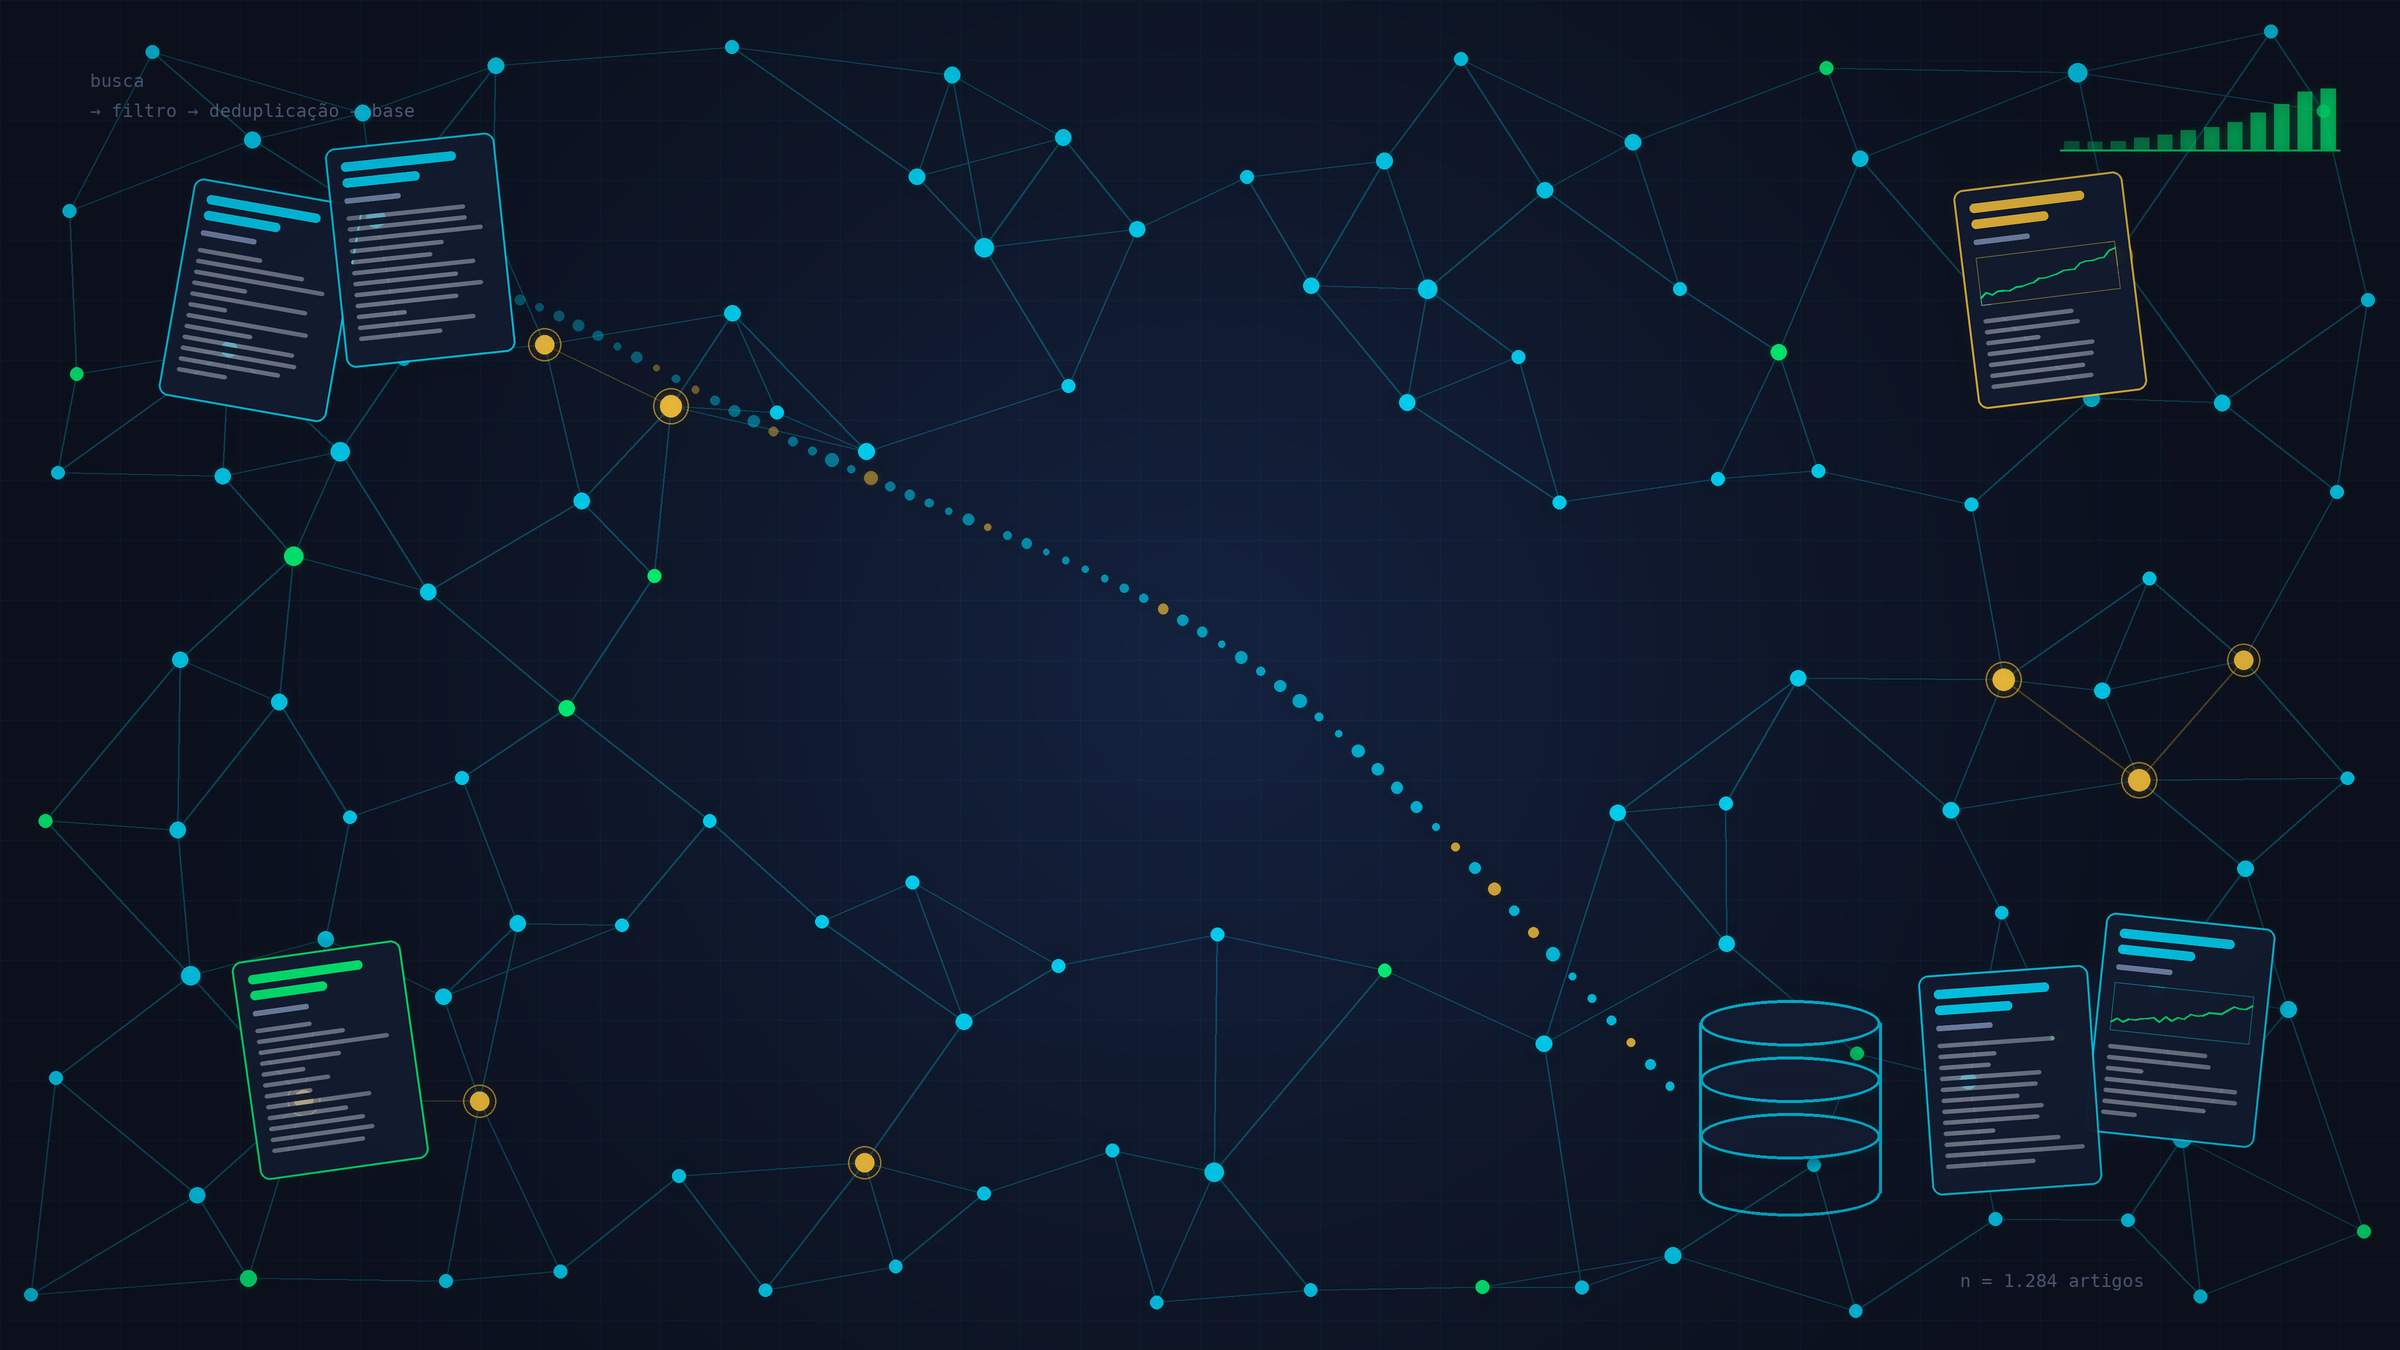
\includegraphics[width=\paperwidth, height=\paperheight]{background.jpeg}
      };
      \fill[bgdark, opacity=0.45] (current page.south west) rectangle (current page.north east);
      \node[font=\LARGE\bfseries, text=white, fill=bgdark, fill opacity=0.88, text opacity=1, inner sep=12pt, rounded corners=8pt, draw=radarcyan!70, line width=1pt, align=center]
        at ([yshift=0.1cm]current page.center) {\insertsectionhead};
    \end{tikzpicture}
  \end{frame}
}

% ── Pacotes ───────────────────────────────────────────────────
\usepackage[brazil]{babel}
\usepackage{amsmath, amssymb, bm}
\usepackage{graphicx}
\usepackage{booktabs}
\usepackage{colortbl}
\usepackage{array}
\usepackage{tikz}
\usetikzlibrary{arrows.meta, positioning, calc, fit, backgrounds}

% ── Estilos TikZ ─────────────────────────────────────────────
\tikzset{
  radarbox/.style={draw=#1!80, rounded corners, fill=#1!15!bgdark, minimum width=2.8cm, minimum height=0.65cm, font=\scriptsize, align=center, text=textmain},
  radararr/.style={-{Stealth[length=2mm]}, thick, radarcyan!60},
  ent/.style={radarbox=#1, minimum width=2.1cm, minimum height=0.7cm, font=\scriptsize, inner sep=2pt},
  proc/.style={radarbox=#1, minimum width=2.2cm, minimum height=1.05cm, font=\footnotesize\bfseries, line width=0.9pt},
  seta/.style={-{Stealth[length=1.8mm]}, thick, #1!70},
}
\arrayrulecolor{radarcyan!40}

% ── Macros ───────────────────────────────────────────────────
\newcommand{\plotbox}[2]{%
  \tikz\node[draw=radarcyan!45, line width=0.6pt, rounded corners=3pt, fill=white, inner sep=2pt]{\includegraphics[#1]{#2}};%
}
\newcommand{\fig}[2][width=\dimexpr\linewidth-6pt\relax]{\plotbox{#1}{figuras/#2}}
\newcommand{\eqpanel}[1]{\par
  \begin{tikzpicture}
    \node[fill=bgcard, draw=radarcyan!40, line width=0.6pt, rounded corners=4pt,
          text width=\textwidth-12pt, inner sep=6pt, align=left, font=\small]{#1};
  \end{tikzpicture}\par}
\newcommand{\eqc}[1]{{\centering$\displaystyle #1$\par}}
\newcommand{\rot}[2]{\textbf{\textcolor{#1}{#2}}}
\newcommand{\motiv}{\rot{accentgold}{Motivação:}\ }
\newcommand{\pendente}[1]{\textcolor{accentgold}{[\,#1\,]}}
\newcommand{\cab}[1]{\textbf{\textcolor{radarcyan}{#1}}}
\newcommand{\cod}[1]{{\ttfamily\color{radargreen}#1}}
\setbeamerfont{block title}{size=\footnotesize, series=\bfseries}
\addtobeamertemplate{frametitle}{}{\vspace{-6pt}}
\setlength{\leftmargini}{1.1em}
\setlength{\leftmarginii}{1.0em}

\title[\apTitulo]{\apTitulo\\ \small \apSubtitulo}
\author{\apAutores}
\date{\apData}

% ══════════════════════════════════════════════════════════════
\begin{document}

% ── Capa ──────────────────────────────────────────────────────
\begin{frame}[plain,noframenumbering]
  \begin{tikzpicture}[remember picture, overlay]
    \node[anchor=center, inner sep=0pt] at (current page.center) {
      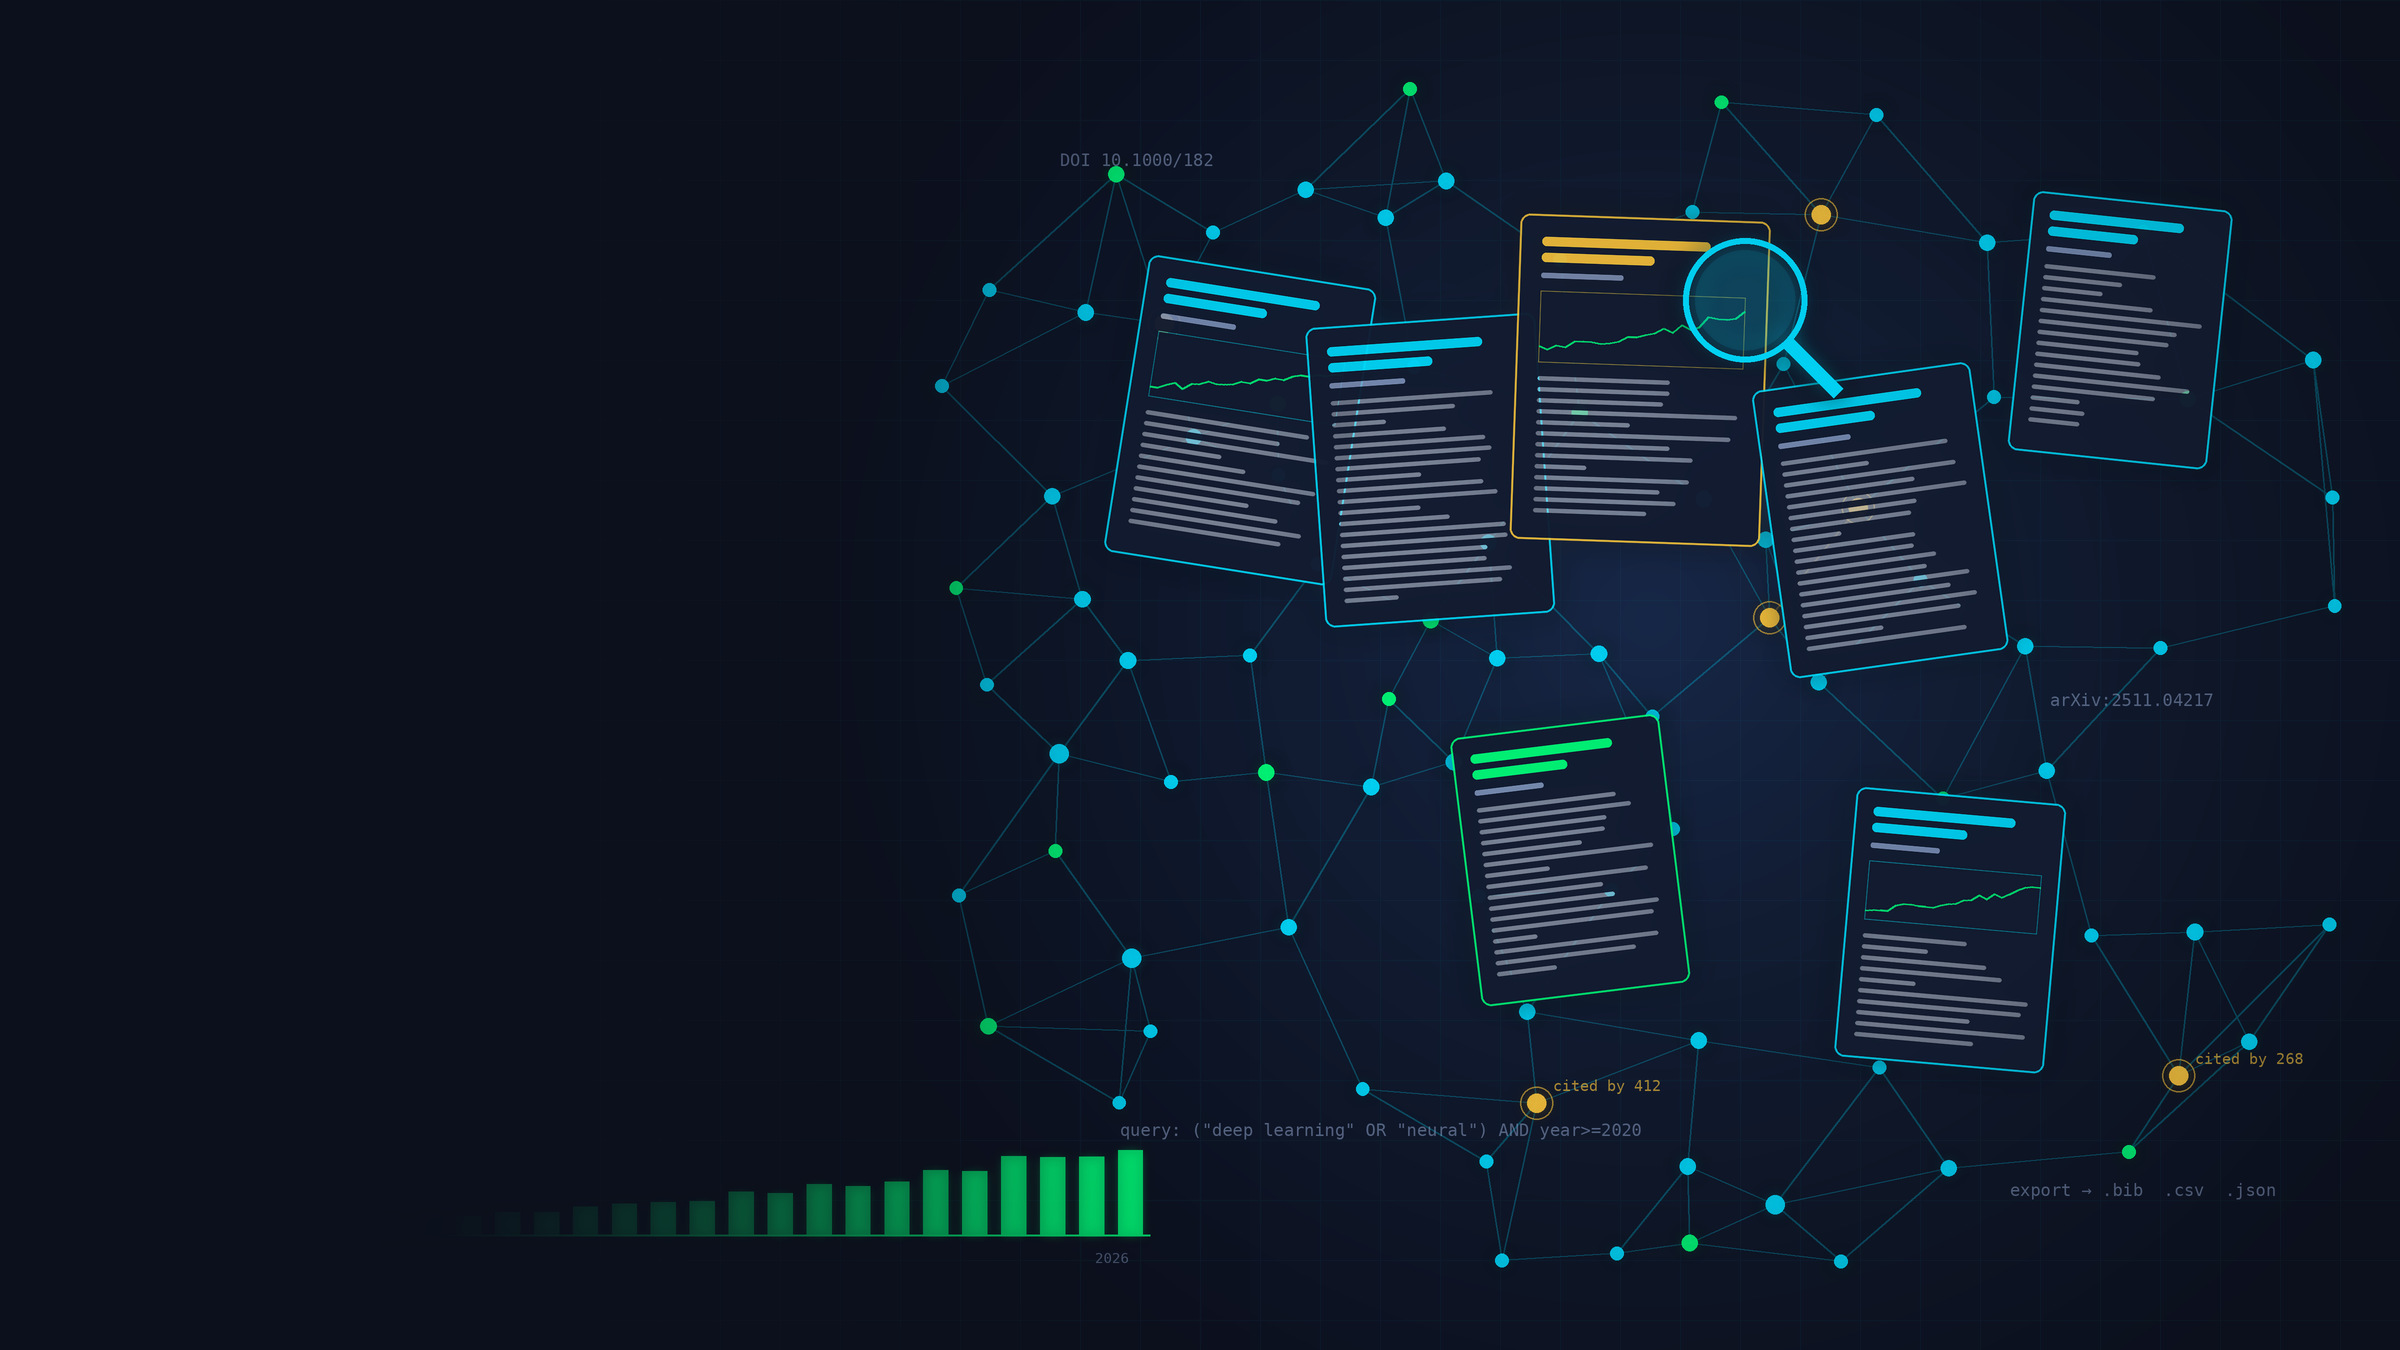
\includegraphics[width=\paperwidth, height=\paperheight]{background_first.jpeg}
    };
    \shade[top color=radarcyan, bottom color=radarcyan!5!bgdark, opacity=0.8]
      ([xshift=1.0cm, yshift=-0.8cm]current page.north west) rectangle ++(0.08cm,-6.8cm);
    \node[anchor=south west, font=\fontsize{22}{27}\selectfont\bfseries, text=white, text width=7.5cm, align=left]
      at ([xshift=1.5cm, yshift=1.15cm]current page.west) {\apTitulo};
    \node[anchor=west, font=\small, text=textsub, text width=7.5cm, align=left]
      at ([xshift=1.5cm, yshift=0.65cm]current page.west) {\apSubtitulo};
    \shade[left color=radarcyan, right color=radarcyan!5!bgdark]
      ([xshift=1.5cm, yshift=0.15cm]current page.west) rectangle ++(6.5cm,0.04cm);
    \node[anchor=west, font=\footnotesize, text=radarcyan, text width=7.5cm, align=left]
      at ([xshift=1.5cm, yshift=-0.45cm]current page.west) {\apAutores};
    \node[anchor=west, font=\footnotesize, text=textsub, text width=7.5cm, align=left]
      at ([xshift=1.5cm, yshift=-1.05cm]current page.west) {\apInstituicao};
    \node[anchor=west, font=\scriptsize, text=textsub!70, text width=7.5cm, align=left]
      at ([xshift=1.5cm, yshift=-1.55cm]current page.west) {\apData};
    \shade[left color=radarcyan!40, right color=accentblue!40]
      ([yshift=0.5cm]current page.south west) rectangle ([yshift=0.54cm]current page.south east);
  \end{tikzpicture}
\end{frame}

% ── Sumário ───────────────────────────────────────────────────
\begin{frame}[t]{Sumário}
  \small
  \tableofcontents
\end{frame}

% ══════════════════════════════════════════════════════════════
\section{Visão geral}
% ══════════════════════════════════════════════════════════════

\begin{frame}[t]{Motivação e objetivo}
  \small
  \motiv uma revisão bibliográfica exige repetir a mesma busca em várias bases, cada uma com sintaxe, limites de taxa e formato de resposta próprios, e depois juntar, deduplicar e triar centenas de resultados à mão.

  \vspace{6pt}
  \begin{columns}[T,onlytextwidth]
    \begin{column}{0.48\textwidth}
      \begin{block}{O que o coletor faz}
        \footnotesize
        \begin{itemize}\setlength{\itemsep}{2pt}
          \item Recebe \textbf{uma} consulta booleana e a traduz para cada base.
          \item Busca em paralelo em 8 APIs acadêmicas.
          \item Grava um CSV por base e um \cod{consolidado.csv} sem duplicatas.
          \item Classifica cada artigo com um LLM local e gera \cod{ranking.csv}.
        \end{itemize}
      \end{block}
    \end{column}
    \begin{column}{0.48\textwidth}
      \begin{exampleblock}{Princípios de projeto}
        \footnotesize
        \begin{itemize}\setlength{\itemsep}{2pt}
          \item Uma base que falha nunca derruba a execução.
          \item Respeito aos limites de cada API (taxa adaptativa).
          \item Segredos só no \cod{.env}, nunca em logs ou CSVs.
          \item Triagem sem enviar dados a serviços externos (Ollama).
        \end{itemize}
      \end{exampleblock}
    \end{column}
  \end{columns}
\end{frame}

\begin{frame}[t]{Arquitetura em dois blocos}
  \centering
  \begin{tikzpicture}[node distance=0.2cm]
    % ── Etapa 1: aquisição ──
    \node[ent=radarcyan] (kw)  at (1.05, 2.5)  {Palavras-chave\\(consulta)};
    \node[ent=radarcyan] (web) at (1.05, 1.15)  {Interface web\\ou \texttt{config.yaml}};
    \node[ent=radarcyan] (bas) at (1.05, -0.2)  {Bases de pesquisa\\(8 APIs)};
    \node[ent=radarcyan] (lim) at (1.05, -1.55) {Limites\\(máx., timeout)};
    \node[proc=radarcyan] (api) at (3.9, 0.5) {Script de\\consumo das APIs};
    \node[proc=radarcyan, minimum width=1.6cm] (lst) at (6.25, 0.5) {Lista de\\artigos};
    \node[font=\tiny, text=textsub, below=0.08cm of lst] {\texttt{consolidado.csv}};
    \foreach \n in {kw, web, bas, lim} \draw[seta=radarcyan] (\n.east) -- (api.west);
    \draw[seta=radarcyan] (api) -- (lst);

    % ── Etapa 2: classificação ──
    \node[ent=accentgold, minimum width=1.95cm] (cri) at (8.85, 2.5)  {Critérios /\\definições};
    \node[ent=accentgold, minimum width=1.95cm] (par) at (11.0, 2.5) {Parâmetros do\\ranking (pesos)};
    \node[ent=accentgold, minimum width=1.95cm] (tmp) at (13.15, 2.5) {Temperatura\\do modelo};
    \node[proc=accentgold, minimum width=2.5cm] (mod) at (9.6, 0.5) {Modelo de\\classificação};
    \node[font=\tiny, text=textsub, below=0.08cm of mod] {Ollama \(\cdot\) \texttt{qwen3.5:0.8b}};
    \node[proc=accentgold, minimum width=1.6cm] (rnk) at (12.4, 0.5) {Ranking\\\texttt{.csv}};
    \node[proc=accentgold, minimum width=2.1cm] (gra) at (12.4, -1.55) {Gráficos /\\grafo web};
    \draw[seta=accentgold] (cri.south) -- (mod.north west);
    \draw[seta=accentgold] (par.south) -- (mod.north);
    \draw[seta=accentgold] (tmp.south) -- (mod.north east);
    \draw[seta=accentgold] (lst.east) -- (mod.west);
    \draw[seta=accentgold] (mod) -- (rnk);
    \draw[seta=accentgold] (rnk) -- (gra);

    % ── Molduras das etapas (mesma altura) ──
    \begin{scope}[on background layer]
      \node[draw=radarcyan!70, fill=radarcyan!7!bgdark, rounded corners=6pt, line width=0.8pt, inner sep=7pt,
            fit=(kw)(lim)(api)(lst)(gra.south -| lst),
            label={[font=\small\bfseries, text=radarcyan]above:1 \(\cdot\) AQUISIÇÃO}] (f1) {};
      \node[draw=accentgold!80, fill=accentgold!7!bgdark, rounded corners=6pt, line width=0.8pt, inner sep=7pt,
            fit=(cri)(tmp)(mod)(gra)(kw.north -| mod),
            label={[font=\small\bfseries, text=accentgold]above:2 \(\cdot\) CLASSIFICAÇÃO}] (f2) {};
    \end{scope}
    \node[font=\scriptsize, text=textsub, align=center, below=0.15cm of f1]
      {consulta \(\rightarrow\) tradução por base \(\rightarrow\) paginação\\normalização \(\rightarrow\) enriquecimento \(\rightarrow\) deduplicação};
    \node[font=\scriptsize, text=textsub, align=center, below=0.15cm of f2]
      {título + resumo + critérios \(\rightarrow\) aderência (0; 0,5; 1)\\com citação literal do resumo \(\rightarrow\) score \(\rightarrow\) ranking};
  \end{tikzpicture}
\end{frame}

% ══════════════════════════════════════════════════════════════
\section{Etapa 1 -- Aquisição}
% ══════════════════════════════════════════════════════════════

\begin{frame}[t]{Bases consultadas}
  \footnotesize
  \renewcommand{\arraystretch}{1.18}
  \centering
  \begin{tabular}{@{}l l l l@{}}
    \toprule
    \cab{Base} & \cab{Interface} & \cab{Credencial} & \cab{Taxa (req/s)} \\
    \midrule
    OpenAlex         & REST JSON, \texttt{cursor}            & \texttt{OPENALEX\_API\_KEY} (obrigatória) & 10 \\
    Semantic Scholar & REST JSON + \texttt{/paper/batch} & \texttt{S2\_API\_KEY} (opcional)          & 1 \\
    Crossref         & REST JSON, \texttt{offset}            & e-mail (pool \emph{polite})              & 3 (1 sem e-mail) \\
    arXiv            & Atom XML                              & nenhuma                                  & 0,33 \\
    PubMed           & E-utilities (\texttt{esearch}+\texttt{efetch}) & \texttt{NCBI\_API\_KEY} (opcional) & 3 (9 com chave) \\
    Europe PMC       & REST JSON, \texttt{cursorMark}        & nenhuma                                  & 2 \\
    CORE             & REST JSON, \texttt{offset}            & \texttt{CORE\_API\_KEY} (opcional)        & 0,5 (2 com chave) \\
    DOAJ             & Lucene, até 1.000 resultados          & nenhuma                                  & 2 \\
    \midrule
    \textcolor{textsub}{OpenCitations} & \textcolor{textsub}{enriquecedor (referências, citações)} & \textcolor{textsub}{token opcional} & \textcolor{textsub}{3} \\
    \bottomrule
  \end{tabular}

  \vspace{6pt}
  \raggedright
  \textcolor{textsub}{SciELO foi avaliada e desabilitada: a API não tem busca por palavra-chave e o portal de busca proíbe robôs (\texttt{robots.txt}).}
\end{frame}

\begin{frame}[t]{Consulta, paralelismo e limites de taxa}
  \small
  \begin{columns}[T,onlytextwidth]
    \begin{column}{0.5\textwidth}
      \cab{Uma consulta, oito dialetos}
      \begin{itemize}\setlength{\itemsep}{1pt}\footnotesize
        \item Sintaxe única: aspas, \texttt{AND}/\texttt{OR}, parênteses.
        \item Ex.: \texttt{SAR AND Agricultura} vira \texttt{all:SAR AND all:Agricultura} no arXiv e \texttt{query.bibliographic=SAR Agricultura} no Crossref.
        \item Filtros (ano, tipo, idioma, acesso aberto) nativos quando a base suporta; senão, aplicados localmente.
      \end{itemize}
      \vspace{4pt}
      \cab{Orquestração}
      \begin{itemize}\setlength{\itemsep}{1pt}\footnotesize
        \item Uma tarefa \texttt{asyncio} por base; falha isolada.
        \item CSV gravado em lotes, à medida que as páginas chegam.
        \item Cache HTTP em disco por 24 h.
      \end{itemize}
    \end{column}
    \begin{column}{0.47\textwidth}
      \begin{block}{Limitador adaptativo (por base)}
        \footnotesize
        \begin{itemize}\setlength{\itemsep}{2pt}
          \item \emph{Token bucket} + semáforo de concorrência.
          \item \textbf{429}: taxa cai pela metade; respeita \texttt{Retry-After}.
          \item \textbf{5xx / timeout}: backoff exponencial com \emph{jitter}.
          \item Até 6 tentativas por página; depois, status \texttt{parcial}.
          \item +25\,\% após 20 sucessos seguidos, sem passar da taxa inicial.
          \item Prazo global: \texttt{timeout\_pesquisa\_s} (300 s na interface).
        \end{itemize}
      \end{block}
    \end{column}
  \end{columns}
\end{frame}

\begin{frame}[t]{Normalização, enriquecimento e consolidação}
  \small
  \begin{columns}[T,onlytextwidth]
    \begin{column}{0.31\textwidth}
      \cab{Normalização}
      \begin{itemize}\setlength{\itemsep}{1pt}\scriptsize
        \item Cada resposta é mapeada para um esquema único de colunas.
        \item Mapeamento escrito a partir de respostas reais gravadas no teste prático.
        \item Resumo em texto plano; idioma em ISO 639-1.
      \end{itemize}
    \end{column}
    \begin{column}{0.31\textwidth}
      \cab{Enriquecimento}
      \begin{itemize}\setlength{\itemsep}{1pt}\scriptsize
        \item Referências nativas quando a base informa.
        \item IDs OpenAlex convertidos para DOI em lote.
        \item OpenCitations: referências e contagem de citações.
        \item Texto completo (CORE com chave, Europe PMC OA).
      \end{itemize}
    \end{column}
    \begin{column}{0.33\textwidth}
      \cab{Consolidação}
      \begin{itemize}\setlength{\itemsep}{1pt}\scriptsize
        \item Mesmo artigo: DOI, PMID, PMCID ou ID arXiv iguais, ou título ($\geq$ 5 palavras) + ano.
        \item Registros fundidos numa só linha, com prioridade por base.
        \item Só entram artigos com DOI \textbf{e} resumo.
        \item Saída: \cod{consolidado.csv}, 16 colunas.
      \end{itemize}
    \end{column}
  \end{columns}
  \vspace{8pt}
  \eqpanel{\footnotesize\textcolor{textsub}{Saídas de cada execução:}\enskip
    \cod{<base>.csv}\enskip$\cdot$\enskip\cod{consolidado.csv}\enskip$\cdot$\enskip\cod{relatorio.md/.json}\enskip$\cdot$\enskip\cod{execucao.log}\enskip$\cdot$\enskip\cod{config\_usada.yaml}}
\end{frame}

% ══════════════════════════════════════════════════════════════
\section{Etapa 2 -- Classificação}
% ══════════════════════════════════════════════════════════════

\begin{frame}[t]{Triagem com LLM local}
  \small
  \begin{columns}[T,onlytextwidth]
    \begin{column}{0.5\textwidth}
      \cab{Para cada linha do consolidado}
      \begin{enumerate}\setlength{\itemsep}{2pt}\footnotesize
        \item Monta o \emph{prompt} com critérios, título, resumo e palavras-chave.
        \item O modelo (Ollama, padrão \texttt{qwen3.5:0.8b}) devolve JSON estruturado: justificativa, citação e aderência.
        \item A citação precisa aparecer \textbf{literalmente} no resumo; senão, a resposta é rejeitada.
        \item Falha num artigo vira \texttt{llm\_status=erro} e não interrompe os demais.
      \end{enumerate}
    \end{column}
    \begin{column}{0.47\textwidth}
      \begin{block}{Aderência aos critérios}
        \footnotesize
        \renewcommand{\arraystretch}{1.15}
        \begin{tabular}{@{}l l@{}}
          \texttt{llm\_match = 1}   & \texttt{incluido} \\
          \texttt{llm\_match = 0,5} & \texttt{duvidoso} \\
          \texttt{llm\_match = 0}   & \texttt{excluido} \\
        \end{tabular}
      \end{block}
      \vspace{2pt}
      \begin{exampleblock}{Parâmetros na interface}
        \footnotesize
        \begin{itemize}\setlength{\itemsep}{1pt}
          \item Critérios de inclusão e exclusão (texto livre).
          \item Temperatura de 0 a 1 (padrão 0,1; 0 = reprodutível).
          \item Modelo escolhido entre os instalados no Ollama.
        \end{itemize}
      \end{exampleblock}
    \end{column}
  \end{columns}
\end{frame}

\begin{frame}[t]{Score do ranking}
  \small
  \eqpanel{\eqc{\text{score} = w_a\,\underbrace{m}_{\text{aderência}} + w_r\,\underbrace{\hat{y}}_{\text{recência}} + w_c\,\underbrace{\hat{c}}_{\text{citações/ano}} + w_t\,\underbrace{v_{\text{tipo}}}_{\text{tipo}}}
    \vspace{2pt}
    \eqc{\text{padrão:}\quad \text{score} = 0{,}70\,m + 0{,}10\,\hat{y} + 0{,}10\,\hat{c} + 0{,}10\,v_{\text{tipo}}}
    \vspace{2pt}
    \eqc{\hat{c} = \operatorname{minmax}\!\left(\log\!\left(1 + \frac{n_{\text{citações}}}{\text{ano atual} - \text{ano} + 1}\right)\right)}}
  \vspace{4pt}
  \begin{columns}[T,onlytextwidth]
    \begin{column}{0.5\textwidth}
      \begin{itemize}\setlength{\itemsep}{2pt}\footnotesize
        \item Pesos padrão: $w_a = 0{,}70$ e $w_r = w_c = w_t = 0{,}10$.
        \item Ajustáveis por execução: somam 100\,\%, aderência $\geq$ 50\,\%.
        \item Recência e citações: min-max entre os artigos do consolidado.
        \item Dado ausente (ano, citações ou tipo) recebe valor neutro 0,5.
      \end{itemize}
    \end{column}
    \begin{column}{0.47\textwidth}
      \footnotesize
      \cab{Valor por tipo de publicação (padrão)}\par\vspace{2pt}
      \renewcommand{\arraystretch}{1.05}
      \begin{tabular}{@{}l r@{\hspace{18pt}}l r@{}}
        artigo      & 1,0 & livro/capítulo & 0,6 \\
        revisão     & 1,0 & preprint       & 0,5 \\
        conferência & 0,8 & outros         & 0,4 \\
      \end{tabular}
      \par\vspace{4pt}
      \textcolor{textsub}{\cod{ranking.csv} = 16 colunas do consolidado + \texttt{llm\_label}, \texttt{llm\_match}, \texttt{llm\_justification}, \texttt{llm\_score}, \texttt{llm\_status}, ordenado por score.}
    \end{column}
  \end{columns}
\end{frame}

% ══════════════════════════════════════════════════════════════
\section{Resultados e conclusão}
% ══════════════════════════════════════════════════════════════

\begin{frame}[t]{Execução real: \texttt{SAR AND Agricultura}}
  \footnotesize
  \begin{columns}[T,onlytextwidth]
    \begin{column}{0.49\textwidth}
      \centering
      \cab{Artigos gravados por base}\par\vspace{2pt}
      \fig[width=0.94\linewidth]{bases_gravados.pdf}
    \end{column}
    \begin{column}{0.49\textwidth}
      \centering
      \cab{Funil da consolidação}\par\vspace{2pt}
      \fig[width=0.94\linewidth]{funil\_consolidacao.pdf}
    \end{column}
  \end{columns}
  \vspace{4pt}
  \raggedright
  Execução de 31/10/2026, 100 artigos por base, sem filtros: 197 s no total; 15 artigos encontrados em 2 ou mais bases.
  OpenAlex e Semantic Scholar falharam (HTTP 401 por chave e HTTP 429) sem interromper as outras seis bases.
  Distribuição de rótulos do ranking: \pendente{executar a triagem LLM nesta consulta e incluir o resultado}.
\end{frame}

\begin{frame}[t]{Limitações e conclusão}
  \small
  \begin{columns}[T,onlytextwidth]
    \begin{column}{0.48\textwidth}
      \begin{alertblock}{Limitações}
        \footnotesize
        \begin{itemize}\setlength{\itemsep}{2pt}
          \item Bases sem chave (Semantic Scholar) sofrem 429 com frequência.
          \item Mesma referência pode aparecer como DOI e como \texttt{pmid:}.
          \item Triagem usa só título e resumo; modelo pequeno pode errar.
          \item Precisão da triagem: \pendente{comparar com rotulação manual}.
        \end{itemize}
      \end{alertblock}
    \end{column}
    \begin{column}{0.48\textwidth}
      \begin{exampleblock}{Conclusão}
        \footnotesize
        \begin{itemize}\setlength{\itemsep}{2pt}
          \item Uma consulta alimenta 8 bases em paralelo, com falhas isoladas.
          \item Resultado único e deduplicado em \cod{consolidado.csv}.
          \item Triagem local e auditável: cada decisão traz uma citação do resumo.
          \item Ranking configurável e grafo de referências na interface web.
        \end{itemize}
      \end{exampleblock}
    \end{column}
  \end{columns}
  \vspace{10pt}
  \centering
  {\large\bfseries\textcolor{white}{Obrigado!}}\par
  \vspace{2pt}
  \textcolor{textsub}{\footnotesize Código e especificação: \texttt{README.md} e \texttt{ESCOPO.md} do repositório.}
\end{frame}

\end{document}
